%!TeX root = Chapter_Introduction2
\documentclass[../../CompleteThesis2/Complete_2ndDraft]{subfiles}
%\graphicspath{{../../Figures/}}
\begin{document}
%	\todo{INTRO: References missing in entire section}
The introduction to this work contains a motivation on why the research is of relevance, on what basis the general idea is based upon, and how the method is carried out. Along with this, it contains a brief walk through of the content of the entire thesis, and a short description of what software was developed, and where it is available.
\minitoc	

\section[Ice Cores]{Ice Cores as a Window to the Past}
\label{Sec:StudyIceCores}

The studies of ice cores have revealed much information and knowledge about the dynamics of the world's past climate, atmosphere and geology through measured proxies such as isotopic \cite[W. Dansgaard, 1964]{Dansgaard1964}, \cite[S. Johnsen et al., 2001]{Johnsen2001} and chemical compositions, conductivity \cite[Moore et al., 1990]{Moore1990}, and dust measurements \cite[F. Lambert et al., 2008]{Lambert2008}. By disclosing information about our past, the analysis of ice cores leads us to a greater understanding of the behaviors of the Earth system, which opens up for possibilities of modeling and predicting the future that lies ahead of us.
	
When analyzing ice cores it is most important that a relationship between depth and age is accurately established, as these timescales are of the essence when building empirical models and reconstructing paleoenvironments \cite[E. Capron, 2013]{Capron2013}. Dating of ice cores can be attempted through a variety of methods: visual inspection of annual layers in data, known volcanic events detected in the ice \cite[B. M. Vinther et al., 2006]{Vinther2006} or radiocarbon dating \cite[S. Aciego et al., 2011]{Aciego2011}, to name a few. 
	
A difficulty, that arises when dating ice cores, is the effects of diffusion through the firn column. Both gas and water molecules can diffuse through the firn which presents a number of obstacles for the continued dating. Firstly, the diffusion of gases in firn, through air pockets connected to the atmosphere, makes the age of the gas in the ice younger than the age of the firn at the same depth. Secondly, the diffusion of solid state molecules present in the firn, like water molecules, erases some of the signal, when measuring different properties of the ice. This erasure is commonly described through the average diffusion length of a molecule at a given depth, $\sigma$. This work focuses in particular on the densification and diffusion processes affecting water isotopic ratios in the firn.
	
The diffusion length $\sigma$ is affected by a variety of parameters: the depth, the annual average accumulation, the ice flow and - especially interesting - the temperature \cite[C. Holme et al., 2018]{Holme2018}. By understanding which parameters influence the behavior of $\sigma$, it might be possible to use this signal erasure obstacle to gain more knowledge about paleoconditions: if it is possible to empirically estimate a diffusion length at a given depth, it may be achievable to reconstruct the temperature for this time interval.

The goal of this thesis is to establish a method for estimating the diffusion length for a given depth section. This is achieved through different analyses, and through a hidden gem in the ice cores.
	
\section[A Rare Gem]{A Rare Gem of Knowledge}
\label{Sec:RareGem}
\begin{figure}
	\centering
	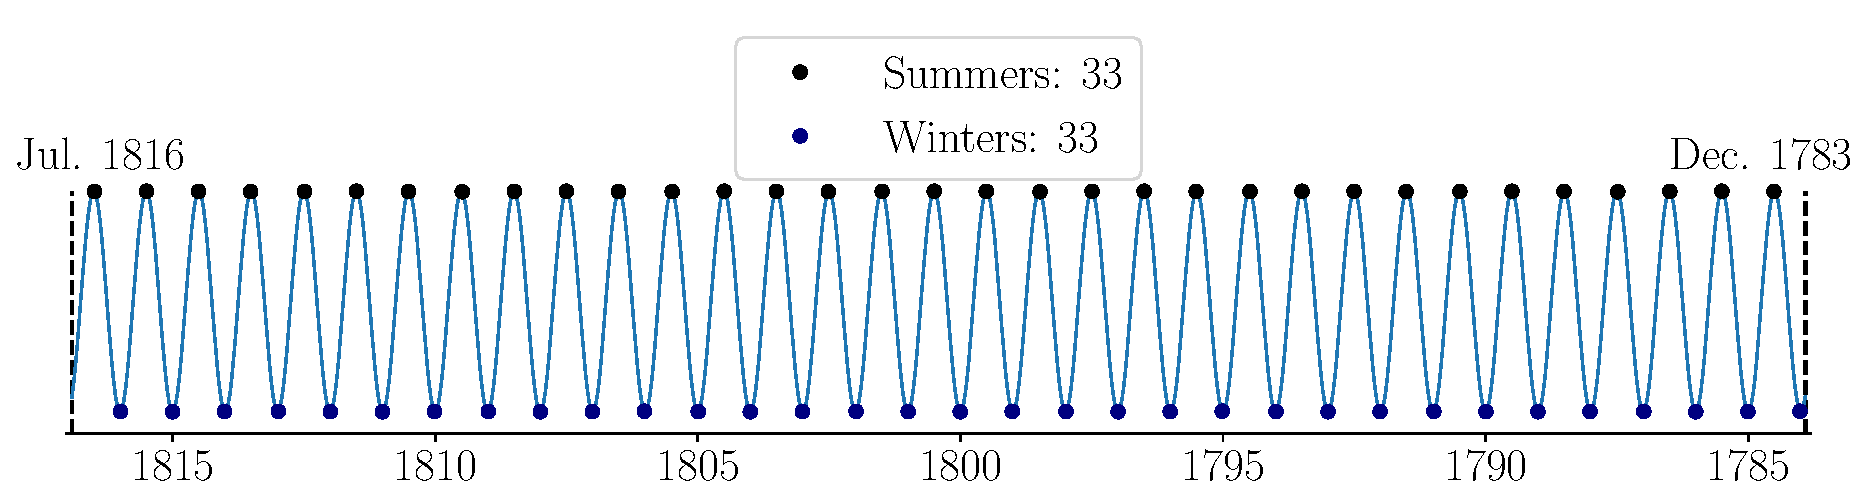
\includegraphics[width=\textwidth]{summersWinters_LT.pdf}
	\caption[Summers and Winters between Laki and Tambora]{Visualization of pattern of summers and winters in the time span between the Laki and Tambora volcanic depositions in Greenland.}
	\label{Fig:LakiTamb_SummerWinter}
\end{figure}
	
In June 1783 the Icelandic volcano Laki erupted explosively \cite[J. Steingrímsson, 1998]{Steingrimsson1998}. The eruption led to an eight-month long emission of volcanic aerosols into the European airspace, bringing climatic and sociological disruptions with it \cite[R. Stone, 2004]{Stone2004}, \cite[T. Thordaldson and S. Self, 2004]{Thordaldson2004}. Although a cataclysmic catastrophe for much of Europe, with extreme weather, famine and higher death rates, the violence of the impact on the life of Europeans, led to this eruption being very well documented and recorded across most of Europe. \\
Later, in April of 1815 on the Southern Hemisphere, the eruption of the Indonesian volcano Tambora resulted in a series of events just as, or even more fatal than, the Laki eruption \cite[C. Oppenheimer, 2003]{Oppenheimer2003}. Tens of or even hundreds of thousands died either during the eruption or in direct consequences hereof, from starvation or epidemic diseases. Furthermore, the eruption, following a number of decades with heavy volcanic activity \cite[J. Cole-Dai et al., 2009]{Dai2009}, left its mark on the climate of the entire Earth system, disrupting global temperatures. In Europe, the following year of 1816 became knwon as \textit{The Year Without a Summer} \cite{Oppenheimer2003}, and the apocalyptic climate affected not only the crops and human necessities, but also the artistic and sociological environment of Europe. Writers like Lord Byron (\textit{Darkness} 1816, \ref{Verse:Darkness}) and Mary W. Shelley (\textit{Frankenstein} 1815-1818) became inspired by the cold and dark weather \cite[A. Marshall, 2020]{Marshall2020}, and painter J. M. W. Turner was clearly influenced by the change of colour of the world, to a more yellow, brown and gloomy ambiance of the 1816 European summer, for example in the painting \textit{The Eruption of the Soufriere Mountains in the Island of St Vincent, 30 April 1812}, 1815, see Figure \ref{Fig:Turner} \cite[C. Zerefos, 2007]{Zerefos2007}.

Both volcanic events were not only landmarks in European history, but quite literally also left their marks on the Greenlandic ice sheet, by deposition of volcanic material through precipitation. These layers of snow with extra high content of volcanic material shows to be a rare gem of knowledge, hidden in the ice. When measuring ice cores this can be utilized along with a different property of the data signals available through ice core analysis, namely the seasonality of a given parameter.

Some measured signals in the ice cores contain annual cycles. For example, the water isotopic ratios in the firn are sensitive to temperature \cite[J. Jouzel, 1997]{Jouzel1997}, leading to a clear summer-to-winter cycle. This makes it relatively easy to date shallow ice cores as the cycles can be counted, but as diffusion takes place in the firn column, some of this signal is washed away. Luckily, another method can be utilized to date the ice: detection of known volcanic events through electrical conductivity measurements. This reveals a quite unique gem of knowledge: by knowing the time of a certain volcanic event, either through historical observations or through previous ice core synchronization, and matching this with the depth of the detected event in the ice, it is possible to set some very certain dates on the timescale of the ice. 

An example of this type of event dating, which is used in this work, is by examining the volcanic eruptions of Laki and Tambora. Both eruptions are, as described, very well historically documented and are visible and detectable in a great number of ice cores \cite[H. Clausen, 1988]{Clausen1988a}, \cite[C. Langway, 1988]{Langway1988}. The deposition in Greenlandic ice cores has been estimated to be in December 1783 for Laki and in July 1816 for Tambora, yielding 33 summers and winters between the two events, see Figure \ref{Fig:LakiTamb_SummerWinter} \cite[J. Cole-Dai et al., 2009]{Dai2009}, \cite[L. Wei, 2008]{Wei2008}. This does not only make it possible to generally date and synchronize different ice cores, but it also allows for in depth analysis of the diffusion and densification processes in the ice.
	

	
	
\section[Using the Rare Gem]{Utilizing the Rare Gem}
\label{Sec:UtilizinGem}
By considering an isotopic depth series situated between two volcanic events, it is possible to back diffuse this series over the known time span in years - or even months - using the diffusion length as a tuning parameter. This is an optimal way to empirically estimate the diffusion length of a given depth interval which makes it possible to obtain a temperature reconstruction of this interval, as $\sigma$ is temperature sensitive \cite{Holme2018}.

The goal is thus to reconstruct the lost signal by a back diffusion scheme, tuning $\sigma$ of the diffusion process, until the known actual number of winters/summers between the events can be counted as peaks and valleys in the depth signal. Then the estimated optimal diffusion length can be used to make a temperature estimate of the given interval.
The back diffusion method is built on both empirical models and signal analysis of the measured data. A simplified flowchart of the general idea is illustrated in Figure \ref{Fig:Flowchart_Intro}.

\begin{figure}[h]
	\begin{tikzpicture}[node distance=1.1cm, auto]
		\node(in1) [io, text width=2.5cm, align=center] {Depth series,\\ $d$};
		\node(in2) [io, text width=3cm,align=center, left of=in1, xshift=-3.5cm] {Core \\specifications};
		\node(in3) [io, right of=in1, text width=2cm,xshift=2.5cm] {Constraints\\for $d$};
		
		\node(pro1) [process, text width=3cm, align=center, below of=in1, yshift=-.5cm] {Signal analysis};
		\node(pro2) [process, text width=3cm, align=center, below of=in2, yshift=-.5cm] {Models};
		\node(pro2pro1) [process, text width=2cm, align=center, below of=pro2, xshift=-1.5cm, yshift=-.3cm, scale=0.9] {Density};
		\node(pro2pro2) [process, text width=2cm, align=center, below of=pro2, xshift=1.5cm, yshift=-.3cm, scale=0.9] {Diffusion};
		
		\node(goal1) [decision, text width=5cm, below of=in1, yshift=-3.1cm, xshift=0cm,] {SIGNAL RESTORATION\\AND ENHANCEMENT};
		
		\node(goal2) [io, text width=3cm, below of=goal1, yshift=-.4cm,] {Optimal $\sigma$ estimate};
		\node(goal3) [io, text width=3cm, right of=goal2, xshift=3cm] {Temperature estimate, $T$};
		
		\draw[arrow] (in2) -- (pro2);
		\draw[arrow] (in1) -- (pro1);
		\draw[arrow] (pro2) -- (pro2pro1);
		\draw[arrow] (pro2) -- (pro2pro2);
		\draw[arrow] (pro1) -- (goal1);
		\draw[arrow] (in3) |- (goal1);
		\draw[arrow] (pro2pro1) |- (goal1);
		\draw[arrow] (pro2pro2) |- (goal1);
		\draw[arrow] (goal1) -- (goal2);
		\draw[arrow] (goal2) -- (goal3);
		%		\node(empty1) [below of=in1, xshift=3.2cm] {Analysis};
		%		\node(pro1) [process, below of=empty1, yshift=-0.3cm, text width=4cm, align=center] {Find optimal $\sigma$ that fulfills constraints};
		%		\node(pro2) [process, below of=pro1, text width=4cm, yshift=-0.5cm, align=center] {Temperature estimate based on $\sigma_{\text{opt}}$};
		%		
		%		\draw[-] (in1) -| (empty1);
		%		\draw[-] (in2) -| (empty1);
		%		\draw[arrow] (empty1) -- (pro1);
		%		\draw[arrow] (pro1) -- (pro2);
	\end{tikzpicture}
	\caption[General idea flowchart]{Illustration of the general idea, restoring signal by tuning the diffusion length until the expected number of years is detectable in the depth interval.}
	\label{Fig:Flowchart_Intro}
\end{figure}

The data under consideration in this thesis is mostly shallow ice cores, namely the Alphabet cores drilled in the vicinity of the 405 m Crête ice core \cite[H. Clausen and C. Hammer, 1988]{ClausenHammer1988}.
\begin{marginfigure}
	\centering
	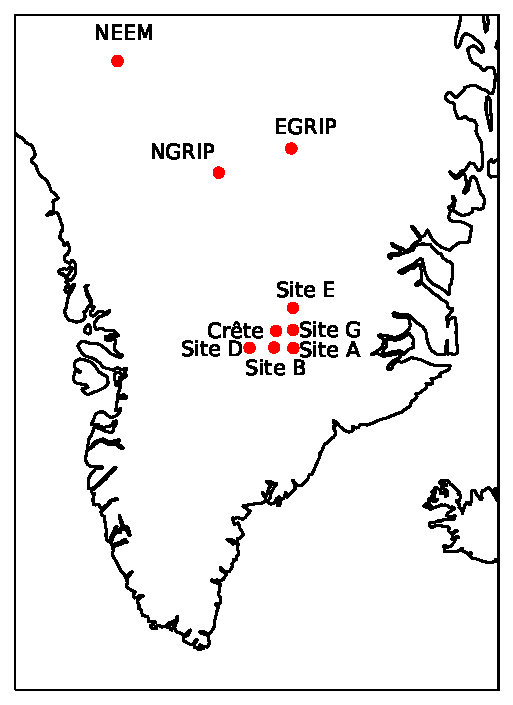
\includegraphics[width=\marginparwidth]{AlphabetCores1.pdf}
	\caption[Map of Greenlandic ice core locations]{\footnotesize Location of Alphabet cores along with some major ice cores, NEEM, EGRIP and NGRIP.}
	\label{Fig:INTRO_AlphabetCoresMap}
\end{marginfigure}
The spatial locations of Crête, the alphabet cores and three other major ice cores, the NEEM \cite{GkinisQuistgaard2021}, NGRIP \cite{NGRIP2014} and EGRIP \cite{EGRIP2016} cores, can be seen in Figure \ref{Fig:INTRO_AlphabetCoresMap}.  


\section[Reading Guide]{Reading Guide}

In this thesis, Chapter \ref{Chap:IceTheory} contains an introduction to the theory of diffusion of water isotopes in ice cores along with theoretical and empirical methods for modeling densification and diffusion profiles. Following, still in Chapter \ref{Chap:IceTheory}, is a brief examination of different experimental methods for detection of deposited volcanic material and which methods have been used for the data under inspection. The chosen data are then presented in Chapter \ref{Chap:Data}, along with an argumentation of why they were selected. Then a thorough presentation of the data and signal analysis along with important computational methods are presented in Chapter \ref{Chap:SigAnalCompMeth}. These different tools are then combined in the method description in Chapter \ref{Chap:MethodAndDiscussion}, depicting a walk-through and testing of the final algorithm developed for estimating the diffusion length given the specific number of years. The final method is tested, and further discussed, developed and fine tuned, still in Chapter \ref{Chap:MethodAndDiscussion}, and results from the final iteration of the method are presented along with a statistical analysis of variations in the final estimates in Chapter \ref{Chap:Results}. On the basis of these results, finally, a basic temperature reconstruction of the examined depth intervals for the ice cores is presented. Finally, a walk through of the most important conclusions and an outlook to future research is given in Chapter \ref{Chap:ConclusionAndOutlook}.

Chapter \ref{Chap:IceTheory} contains already existing material, as it is a walk through of the theory of ice cores developed throughout the last century. Chapter \ref{Chap:Data} contains, as mentioned, a description of data, which is per se not new material, as the ice cores in focus were drilled and analyzed in the 1970's and 1980's, but some small corrections were made to the estimates of the locations of the volcanic events. Chapter \ref{Chap:SigAnalCompMeth} contains a presentation of the existing computational methods utilized, but also a walk through of how the choices of methods and parameters affect the final method. In Chapter \ref{Chap:MethodAndDiscussion} the newly developed back diffusion method is presented along with a discussion of various subjects in the thesis. 

\section[Software]{Software}
All computational analysis carried out in this work is implemented through \lstinline[language=Python]|Python v3.8.10|. All code is available on GitHub repository by T. Quistgaard, Master's Thesis, (2021), GitHub repository: https://github.com/TheaQG/AWI \_Bcores\_Analysis.
The main modules implemented are: 
\begin{itemize}
	\item Herron-Langway densification model, Section \ref{Subsubsec:Ice_DiffusionAndDensification_Densification_HLmodel}, in file \lstinline[language=Python]|HL_AnalyticThea_class.py|.
	\item Diffusion length profile model, Section \ref{Sec:Ice_CFM}, in files \lstinline[language=Python]|DiffusionProfiles_calculations.py| and \lstinline[language=Python]|Diffusivity.py|.
	\item Interpolation methods, Sections \ref{Sec:CompMeths_SplinesAndInterpolation} and \ref{Subsec:METH_Interpolation}, in file \lstinline[language=Python]|Interpolation_Class.py|.
	\item Signal attenuation and annual layer thickness estimation, Section \label{Sec:SignalAnalysis_ALT}, in file \lstinline[language=Python]|SignalAttenuation.py|.
	\item Spectral transforms and analysis, along with general deconvolution/back diffusion method, Sections \ref{Sec:SignalAnalysis_SpectralAnalysis}, \ref{Sec:SignalAnalysis_BackDiffusion} and \ref{Subsec:Method_SigmaMethod_Module1}, in file \lstinline[language=Python]|Decon.py|.
	\item The final optimization module, along with the constrained peak detection method, Sections \ref{Subsec:Method_SigmaMethod_Module2} and \ref{Subsec:Meth_PeakDetection_Constrained}, in file \lstinline[language=Python]|BackDiffuse_LT.py|.
	\item Final temperature estimates, Chapter \ref{Chap:Results}, in files \lstinline[language=Python]|sigmaSolver.py| and \lstinline[language=Python]|TemperatureEstimates.py|.
\end{itemize}
The modules are all described in depth in the corresponding sections referred to, and the connections between modules are illustrated in Figures \ref{Fig:FlowchartBackDiffusion} and \ref{Fig:METH_Flowchart_Optimization}. Along with the presented files are a number of files containing code for testing the different modules and for generating the final results.
%	\section{Old}
%	
%	Many analyses of ice cores have mainly focused on the large scale changes happening over hundreds, thousands and tens of thousands of years, [\ref{label}] \todo{INTRO: REFERENCES and examples}.	When considering such large-scale changes, it is acceptable that the dating of the ice core is off by a year or two as the interest is mainly on the general trends over many years and not on individual annual changes. This is rather lucky, as it is rare to have exact and precise dating, especially in older and deeper cores where the annual layer cycles have been extinguished. 
%	
%	
%	The scope of this project though, has a different focus: When examining ice core data for volcanic eruptions through, for example, electrical conductivity measurements, it is sometimes possible to date the ice cores much more accurate and precise. Two aspects are in play here: Firstly, if volcanic eruptions are visible in more than one ice core it is possible to synchronize all measured quantities in these cores by matching their volcanic profiles. This enhances the accuracy of the dating and also presents the possibility to examine more local behaviors of the Earth system as, for example, cross-hemisphere data can be compared. Secondly, if the eruptions have been recorded in human history, the precision of the dating can be highly improved, as these historical records often contain both time, place, duration and other important parameters of the volcanic events. For this project both aspects are considered as the focus is on the volcanic eruptions of the Icelandic volcano Laki in 1783 and the Indonesian volcano Tambora in 1815, which are both very well historically recorded and documented and are both visible in a great number of ice cores. 
%	
%	This reveals a rare gem of knowledge: as the two eruptions are relatively close in time, well documented and detectable in many cores, it is possible to say with high confidence that any data measured and analyzed, be it isotopic, conductivity, chemical ot otherwise, in the ice core section between these two visible eruptions, must in time represent the time span between the deposition of volcanic material at the ice core site. This allows for in depth analysis of the diffusion and densification processes the ice has been through and makes it possible to examine and develop new methods to restore diffused signals and otherwise lost information with high precision and accuracy. This is mainly due to the constraints raised based on the knowledge of deposition time: Since there are 33 years between the volcanic depositions, there must be detected exactly 33 winters and 33 summers in the isotopic signals. Thus, the restoration of the diffused data series can be optimized to fulfill these criteria.
%	
%	All of this presents a way to make more precise local temperature estimates over a shorter time period through the different temperature proxies present in the ice core data.
%\section[Laki and Tambora]{Laki and Tambora in Recorded History}
%In the not-so-distant past two volcanic horizons have been of great importance for this thesis, namely the Laki eruption in 1783 and the Tambora eruption of 1815. Interestingly, these eruptions have not only impacted the geophysical world, but has left their footprints on the history of Man in politics[REFERENCE], sociology[REFERENCE], arts[REFERENCE] and philosophy[REFERENCE]. On the eighth day of June in 1783 a volcanic fissure located in the southern part of Iceland was central for a global climatic change. The fissure Lakagígar or more commonly known as Laki refering to the central mountain, erupted with violent phreagomagmatic explosions due to the basalt magma being exposed to ground water. The eruption was given a Volcanic Explosivity Index(VEI) of 4, corresponding to the magnitude of the much later 2010 Eyjafjallajökull Icelandic eruption. For the next eight months the fissure continued to emit great amounts of sulfuric aerosols into the atmosphere, resulting locally in Iceland in catastrophic mass famine, due to loss of livestock to poisoning, with up to 25 \% of the population dying from starvation and poisoning from the volcanic gasses. Globally, the eruption caused a huge amount of sulfur dioxide to be spewed into the northern hemisphere which led to a global drop in temperatures and a generally more extreme climate. In the European regions the following summer was much warmer than usual with many thunderstorms to follow. The winter of 1783-84 was subsequently extreme, with long periods of continuous frost. In France the late 1780's were marked by several years with droughts in the summer and frost in the winter, which contributed greatly to a rise in poverty and famine, and creating a greater division between the people and the rulers. Along with a growing dismay and distrust in the ruling forces the climatic changes due to Laki and a number of other climatic disruptions the French political situation finally climaxed in the French revolution of 1789. [REFERENCES!!!!]\\
%32 years later on April 5 in 1815 an even more powerful eruption ensued: the eruption of Mount Tambora on the, now, Indonesian island Sumbawa. This eruption had a Volcanic Explosivity Index of 7, which makes it the most powerful in the recorded history of humankind. Considering that the VEI is defined as a logarithmic scale - at least for indices larger than VEI-3 - the Tambora eruption, though located just south of the Equator, impacted the entire globe as well as the European continent in at least the same magnitude as the 32 years prior Laki eruption. Locally, it was estimated to cause at least 10,000 direct deaths and many tens of thousands more due to sulfur dioxid poisoning, famine and disease. In many contexts the year of 1816 following the event became known as "\textit{The Year Without a Summer}", as the ashes from the eruption column dispersed across the world and lowered global temperatures. This significant climate change though was not just a consequence of the Tambora eruption, but was pushed by a number of climatic forcings, some due to several previous volcanic activities around the globe. Combined, these effects coincided in a drop in global temperature by about 0.4 to 0.7 $^{\circ}$C. This climatic change affected the entire globe by disrupting the Indian monsoons, causing a number of failed harvests, laying ground to severe typhus epidemics in southeast Europe and destroying crops and causing potato, oat and what harvest failure, especially in Ireland. Since the eruption had so severe consequences for the day to day lives of many people, the aftermath all around the world has been one of the greatest documented in recorded time, with a clear impact on the works of many artists, among them Lord Byron and J. M. W Turner[REFERENCES!!!!]. Although both eruptions caused many a tragedy, there is beauty in using these events as volcanic horizons in ice core records. Given the severity of both eruptions, they have been so well documented in historical records that they make up solid and certain pillars in developing a temporal map of the past life of our ever so active earth. For that and for their brutal beauty they will remain in human history for a great while to come.
	
\end{document}